\documentclass[border=3pt]{standalone}
\usepackage{tikz}
\usetikzlibrary{arrows.meta,calc}
\begin{document}
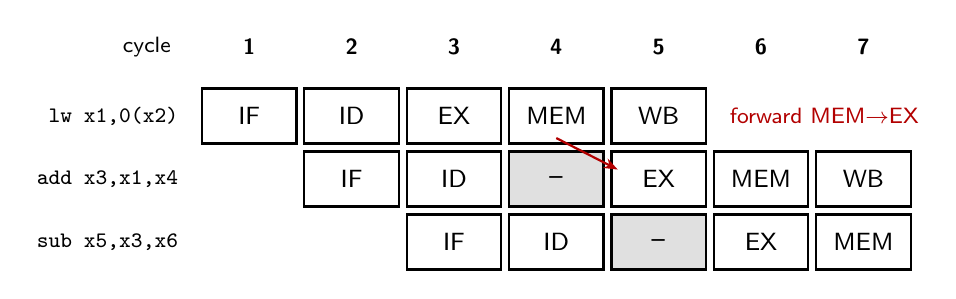
\begin{tikzpicture}[font=\sffamily\small, x=13mm, y=8mm]
  % column headers: cycles
  \foreach \c in {1,...,7}{\node[font=\sffamily\footnotesize\bfseries] at (\c,0.6) {\c};}
  \node[font=\sffamily\footnotesize] at (0,0.6) {cycle};
  % rows
  \node[anchor=east, font=\ttfamily\footnotesize] at (0.4,-0.5) {lw x1,0(x2)};
  \node[anchor=east, font=\ttfamily\footnotesize] at (0.4,-1.5) {add x3,x1,x4};
  \node[anchor=east, font=\ttfamily\footnotesize] at (0.4,-2.5) {sub x5,x3,x6};
  % lw
  \foreach \c/\s in {1/IF,2/ID,3/EX,4/MEM,5/WB}{
    \node[draw, thick, minimum width=12mm, minimum height=7mm] at (\c,-0.5) {\s};}
  % add: stalls in cycle 4 (bubble), EX in 5
  \foreach \c/\s in {2/IF,3/ID}{
    \node[draw, thick, minimum width=12mm, minimum height=7mm] at (\c,-1.5) {\s};}
  \node[draw, thick, fill=black!12, minimum width=12mm, minimum height=7mm] at (4,-1.5) {\textbf{--}};
  \foreach \c/\s in {5/EX,6/MEM,7/WB}{
    \node[draw, thick, minimum width=12mm, minimum height=7mm] at (\c,-1.5) {\s};}
  % sub follows one cycle later
  \foreach \c/\s in {3/IF,4/ID}{
    \node[draw, thick, minimum width=12mm, minimum height=7mm] at (\c,-2.5) {\s};}
  \node[draw, thick, fill=black!12, minimum width=12mm, minimum height=7mm] at (5,-2.5) {\textbf{--}};
  \foreach \c/\s in {6/EX,7/MEM}{
    \node[draw, thick, minimum width=12mm, minimum height=7mm] at (\c,-2.5) {\s};}
  % forward arrow: lw MEM (c4) -> add EX (c5)
  \draw[-{Stealth[length=5pt]}, thick, red!70!black] (4,-0.85) -- (4.6,-1.35);
  \node[font=\sffamily\footnotesize, red!70!black, anchor=west] at (5.6,-0.5) {forward MEM$\to$EX};
\end{tikzpicture}
\end{document}
